%------------------------------------------------------------------------------
%
% Repository path   : $HeadURL: https://hbergauer@forge.hephy.oeaw.ac.at/scm/svn/project-cmstrigger/GlobalTriggerUpgrade/doc/latex/gt-mp7-firmware-specification/content/fdl.tex $
% Last committed    : $Revision: 4475 $
% Last changed by   : $Author: hbergauer $
% Last changed date : $Date: 2018-01-19 10:02:12 +0100 (Fri, 19 Jan 2018) $
% Description       : Specification of Final Decision Logic
% ------------------------------------------------------------------------------
\section{Final Desicion Logic}\label{sec:fdl:ufdl}

The Final Desicion Logic (\ufdl) firmware contains algo-bx-masks, suppression of algos caused by calibration trigger, prescalers, veto-masks and rate-counters
("before prescalers", "after prescalers" and "post dead time") for each Algorithm and the local \finor- and veto-logic.

\begin{figure}[htb]
\centering
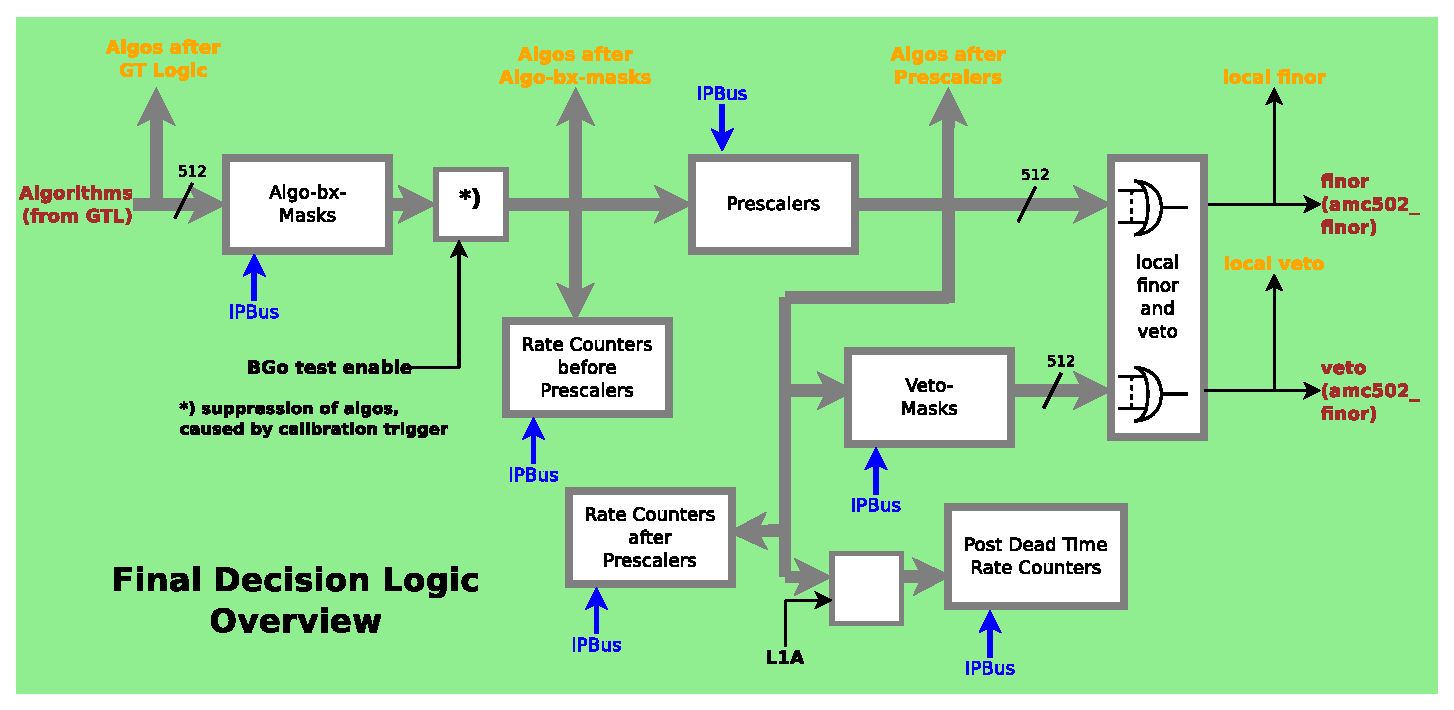
\includegraphics[width=15cm]{figures/mFDL_firmware}
\caption{\ufdl firmware v1.0.1} 
\label{fig:fdl:mFDL_firmware}
\end{figure}

\subsection{\ufdl Interface}
\label{sec:fdl:ufdl_interface}

%\textit{under construction ...}

\textbf{Inputs:}
\begin{itemize}
\item Algorithms from \ugtl
\item IPBus interface (for registers, counters and memories)
\item LHC-clock
\item Reset signal
\item BC0, BGo test-enable, L1A
% \item Indication of LHC gap
\item Begin of lumi-section
% \item Bx-nr for algo-bx-masks memory
\end{itemize}
\textbf{Outputs:}
\begin{itemize}
% \item Status information of \ufdl
\item Prescale factor set index to \rop
\item Algorithms after GTLogic to \rop
\item Algorithms after algo-bx-masks to \rop
\item Algorithms after prescalers to \rop
\item Algorithms after \finor-masks to \rop
\item Local \finor to \rop
\item Local veto to \rop
\item Local \finor with veto to \rop
\item Local \finor to mezzanine
\item Local veto to mezzanine
\item Local \finor with veto to mezzanine
\end{itemize}

\subsection{MP7 \finor hardware solution}

%% Text, figures and tables moved to com-hardware.tex
The firmware of \ufdl in this document is based on a hardware configuration with maximum 6 \ugt modules. 
% A proposed hardware solution for \finor is documented in \ref{sec:com-hard:hw_config_finor_mp7}.

\subsection{Data flow}
\label{sec:fdl:data_flow}

\begin{figure}[htb]
\centering
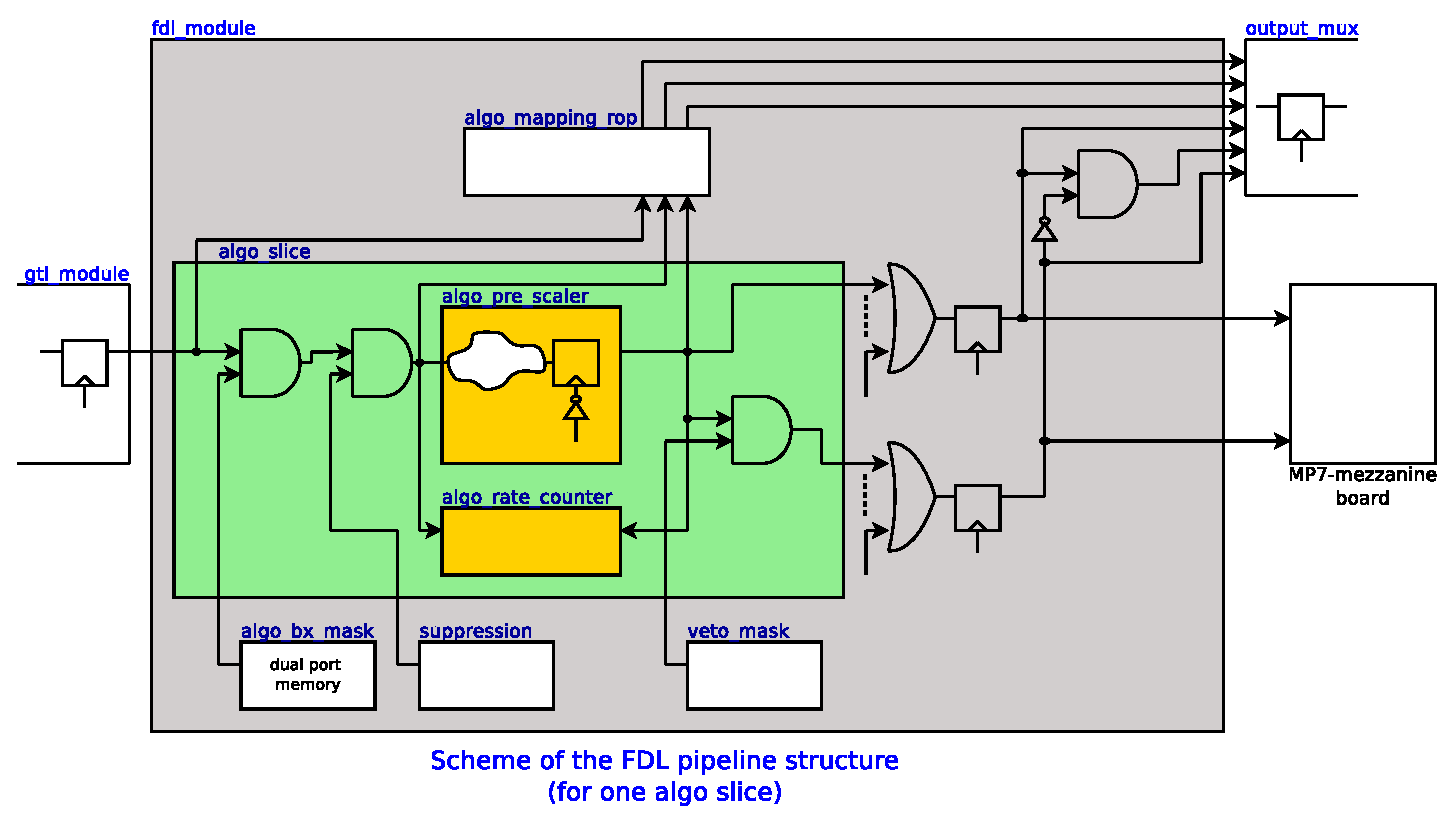
\includegraphics[width=15cm]{figures/fdl_pipeline}
\caption{\ufdl pipeline v1.0.1} 
\label{fig:fdl:mFDL_pipeline}
\end{figure}

Every Algorithm, in total 512 coming from \ugtl, passes a algo-bx-mask, the logic for suppression of algos caused by calibration trigger and a prescaler, which reduces the trigger rate by a given factor. Prescaled Algorithms signals are combined to a local final-or-signal (\finor).
For every Algorithm there is a rate-counter before prescaler and after prescaler, which are incremented by LHC-clock if the Algorithm is true. In addition there are post-dead-time counters, one for each Algorithm, which are incremented,
if the Algorithm and the L1A-signal are true at the same bunch-crossing.
% Algorithms signals after \finor-masks selected by veto-mask disable the total \finor-signal, if one of the selected Algorithm is true. The total \finor-signal is provided to TCDS. 
Algorithms after GTLogic, after algo-bx-masks, after prescalers, the local \finor- and local veto-signal are provided for read-out-record.\\
If there are not enough firmware resources in one \ugt board, more boards could be used. Therefore the 512 Algorithms are partitioned by TME. TME will set the number of Algorithms as
constant in the package module \texttt{gtl\_pkg.vhd}. This means \ugtl and \ufdl firmware considered as a unit for synthesis. In the case of more \ugt boards, the local \finor and local veto are routed via
a mezzanine board on MP7 (located on "General Purpose I/O connector") to the FINOR-AMC502 module, where the total \finor is created and send to TCDS.\\
A mapping for Algorithms is provided, to give flexibility for setting the index of Algorithms:
\begin {itemize}
\item creating a mapping instance (algo\_mapping\_rop.vhd) over TME (see \ref{sec:gtl:algo_mapping_tme}), this component will be instantiated in fix part of FDL, and new calculation will done each time over TME.
\item TME delivers just the number of Algorithms, which will be built on each card.
% \item TME additionally deliver the mapping process, in order FDL and IPBus, ROP know, which algorithm is at which address. 
\item from FDL point of view, FDL see incremented number of Algorithms indexes, \eg 0, 1, 2, which is \eg 69, 200, 300.
\item TME should take care of assignment of each Algorithm to a number, that means if in card 1 algo\_59 is defined, nobody allows to produce the same number again.
\end {itemize}
% A software which manages these partitioned Algorithms for setting prescale factors, reading rate-counters and other accesses has to be developed.\\

\subsection{Main parts}

The top-of-hierarchy module (\texttt{fdl\_module.vhd}) contains 
\begin {itemize}
\item version registers
% \item a control register
\item a command pulse register
% \item a status register
\item prescalers for all Algorithms
\item registers for prescale factors
\item register for prescale factor set index
\item rate-counters for all Algorithms, finor, veto, L1A and post-dead-time
\item read only registers for rate-counter values
\item algo-bx-masks for all Algorithms
\item \finor-masks for all Algorithms
\item veto-masks for all Algorithms
\item the \finor-logic
\end {itemize}

% \subsubsection{Reset structure}
% \label{sec:fdl:reset_structure}
% 
% \textit{under construction ...}
% 
\subsubsection{Registers and memories}
\label{sec:fdl:reg_mem}

All registers and memories are 32 bits wide. (A first draft of the definition of the relative addresses is shown in Table~\ref{tab:ufdl_register_map}.)

\begin {itemize}
\item Dual-port memories for the algo-bx-masks are implemented. For each Algorithm there is a mask bit at every bunch crossing of one orbit. Therefore in total memories of 4096 x 512 bits
are implemented. Because of the 32 bit data interface, 16 memories each with a size of 4096 x 32 bits are instantiated.
\item Read-only registers for the value of rate-counters (before and after prescalers, post-dead-time counters) are implemented, 512 registers, one for every Algorithm. Rate-counter value has 32 bits.
\item Registers for prescale factor of the prescalers are implemented, 512 registers, one for every Algorithm. A prescale factor value has 24 bits.
\item Registers for masks (finor- and veto-masks) are implemented, 512 registers.
\item One register for prescale factors set index is implemented. This register contains a value, which is unique for a given set of prescale factors. The content of this register is
part of \record.
\item One register for command pulses is implemented. One bit of this register (bit 0) is used for "setting the request signal for updating prescale factors high", which enables, that the prescale factors and the prescale factor set index
are loaded at the begin of a luminosity segment period. (Other bits are not defined yet.)
\item One control register is implemented (the content has to be defined).
% \item One register for status information is implemented. The content has to be defined.
\item 32 register for L1 Trigger Menu name for \ugtl is implemented.
\item 4 register for L1 Trigger Menu UUID for \ugtl is implemented.
\item One register for L1 Trigger Menu compiler version is implemented.
\item One register for \ufdl firmware version is implemented.
\item One register for \ugtl firmware (fixed code) version is implemented.
\end {itemize}

\paragraph{Register map}
\label{sec:fdl:reg_map}
The register map for \ufdl has a base address of \verb|0x90000000|.

% % HB 2016-11-03: inserted "longtable"
\begin{longtable}{c p{.4\columnwidth} c p{.33\columnwidth}}
\caption{\ufdl register map}\\
\hline 
Offset & {Register name} & {Access} & {Description}\\
\hline
\hline
\endhead
0x90000000 & \verb|Algo BX masks(0)| & r/w & 4096 memory addresses of algo-bx-masks for Algorithms 0-31.\\
0x90001000 & \verb|Algo BX masks(1)| & r/w & 4096 memory addresses of algo-bx-masks for Algorithms 32-63.\\
... & ... & ... & ...\\
0x9000F000 & \verb|Algo BX masks(15)| & r/w & 4096 memory addresses of algo-bx-masks for Algorithms 480-511.\\
0x90010000 & \verb|Rate counter before prescaler| & r & 512 read-only registers for rate-counter values before prescalers.\\
0x90010200 & \verb|Prescale factors| & r/w & 512 registers for prescale factors.\\
0x90010400 & \verb|Rate counter after prescaler| & r & 512 read-only registers for rate-counter values after prescalers.\\
0x90010600 & \verb|Rate counter post-dead-time| & r & 512 read-only registers for post-dead-time rate-counter values.\\
0x90010800 & \verb|Masks| & r/w & 512 registers for finor-masks and veto-masks. Bit 0 = finor-mask, bit 1 = veto-mask.\\
0x90091880 & \verb|Prescale factors set index| & r/w & Register for prescale factors set index.\\
% 0x90091888 & \verb|Control| & r/w & Register for control signals (content has to be defined !!!).\\
0x900918C0 & \verb|L1tm name| & r & 32 registers for L1 Trigger Menu name for \ugtl.\\
0x900918E0 & \verb|L1tm uuid| & r & 4 registers for L1 Trigger Menu UUID for \ugtl.\\
0x900918E4 & \verb|L1tm compiler version| & r & Register for L1 Trigger Menu compiler version.\\
0x900918E5 & \verb|GTL FW version| & r & Register for firmware version of \ugtl VHDL code.\\
0x900918E6 & \verb|FDL FW version| & r & Register for firmware version of \ufdl VHDL code.\\
0x900918E7 & \verb|L1tm FW uuid| & r & 4 registers for L1 Trigger Menu FW UUID for \ugtl.\\
0x900918EB & \verb|SVN revision number| & r & Register for SVN revision number.\\
0x900918EC & \verb|L1tm uuid hash| & r & Register for L1 Trigger Menu UUID hash for \ugtl.\\
0x900918ED & \verb|L1tm FW uuid hash| & r & Register for L1 Trigger Menu FW UUID hash for \ugtl.\\
0x900918EE & \verb|Module ID| & r & Register for Module ID of L1 Trigger Menu.\\
0x90091900 & \verb|Command Pulses| & r/w & Register for command pulses.\\
0x90091980 & \verb|Rate counter finor| & r & One read-only registers for finor rate-counter value.\\
0x90092200 & \verb|L1A latency delay| & r/w & Register for L1A latency delay value (used for post-dead-time counter).\\
0x90093000 & \verb|Rate counter L1A| & r & One read-only registers for L1A rate-counter value.\\
0x90094000 & \verb|Rate counter veto| & r & One read-only registers for veto rate-counter value.\\
0x90095000 & \verb|Current prescale set index| & r & Read-only register for prescale factors set index, which was "updated" with begin of current lumi-section ("prescale\_factors\_set\_index\_reg\_updated(0)" in VHDL).\\
0x90095001 & \verb|Previous prescale set index| & r & Read-only register for prescale factors set index, which was "updated" with begin of previous lumi-section for monitoring "prescale\_factors\_set\_index\_reg\_updated(1)" in VHDL).\\
0x90096000 & \verb|Calibration trigger gap| & r/w & Register for begin and end (in Bx) of calibration trigger gap.\\
\hline
\label{tab:ufdl_register_map}
\end{longtable}

% \medskip
% \begin{table}[htdp]
% \footnotesize
% \begin{center}
% \begin{tabular}{c p{.4\columnwidth} c p{.33\columnwidth}}
% \toprule
% Offset & {Register name} & {Access} & {Description}\\
% \midrule      
% 0x90000000 & \verb|Algo BX masks(0)| & r/w & 4096 memory addresses of algo-bx-masks for Algorithms 0-31.\\
% % 0x90001000 & \verb|Algo BX masks(1)| & r/w & 4096 memory addresses of algo-bx-masks for Algorithms 32-63.\\
% ... & ... & ... & ...\\
% 0x9000F000 & \verb|Algo BX masks(15)| & r/w & 4096 memory addresses of algo-bx-masks for Algorithms 480-511.\\
% 0x90010000 & \verb|Rate counter before prescaler| & r & 512 read-only registers for rate-counter values before prescalers.\\
% 0x90010200 & \verb|Prescale factors| & r/w & 512 registers for prescale factors.\\
% 0x90010400 & \verb|Rate counter after prescaler| & r & 512 read-only registers for rate-counter values after prescalers.\\
% 0x90010600 & \verb|Rate counter post-dead-time| & r & 512 read-only registers for post-dead-time rate-counter values.\\
% 0x90010800 & \verb|Masks| & r/w & 512 registers for finor-masks and veto-masks. Bit 0 = finor-mask, bit 1 = veto-mask.\\
% 0x90091880 & \verb|Prescale factors set index| & r/w & Register for prescale factors set index.\\
% % 0x90091888 & \verb|Control| & r/w & Register for control signals (content has to be defined !!!).\\
% 0x900918C0 & \verb|L1tm name| & r & 32 registers for L1 Trigger Menu name for \ugtl.\\
% 0x900918E0 & \verb|L1tm uuid| & r & 4 registers for L1 Trigger Menu UUID for \ugtl.\\
% 0x900918E4 & \verb|L1tm compiler version| & r & Register for L1 Trigger Menu compiler version.\\
% 0x900918E5 & \verb|GTL FW version| & r & Register for firmware version of \ugtl VHDL code.\\
% 0x900918E6 & \verb|FDL FW version| & r & Register for firmware version of \ufdl VHDL code.\\
% 0x900918E7 & \verb|L1tm FW uuid| & r & 4 registers for L1 Trigger Menu FW UUID for \ugtl.\\
% 0x900918EB & \verb|SVN revision number| & r & Register for SVN revision number.\\
% 0x900918EC & \verb|L1tm uuid hash| & r & Register for L1 Trigger Menu UUID hash for \ugtl.\\
% 0x900918ED & \verb|L1tm FW uuid hash| & r & Register for L1 Trigger Menu FW UUID hash for \ugtl.\\
% 0x900918EE & \verb|Module ID| & r & Register for Module ID of L1 Trigger Menu.\\
% 0x90091900 & \verb|Command Pulses| & r/w & Register for command pulses.\\
% 0x90091980 & \verb|Rate counter finor| & r & One read-only registers for finor rate-counter value.\\
% 0x90092200 & \verb|L1A latency delay| & r/w & Register for L1A latency delay value (used for post-dead-time counter).\\
% 0x90093000 & \verb|Rate counter L1A| & r & One read-only registers for L1A rate-counter value.\\
% 0x90094000 & \verb|Rate counter veto| & r & One read-only registers for veto rate-counter value.\\
% 0x90095000 & \verb|Prescale factors set index updated 0| & r & Read-only register for prescale factors set index, which was "updated" with begin of current lumi-section ("current\_prescale\_set\_index" in TDF).\\
% 0x90095001 & \verb|Prescale factors set index updated 1| & r & Read-only register for prescale factors set index, which was "updated" with begin of previous lumi-section for monitoring ("previous\_prescale\_set\_index" in TDF).\\
% 0x90096000 & \verb|Calibration trigger gap| & r/w & Register for begin and end (in Bx) of calibration trigger gap.\\
% \bottomrule
% \end{tabular}
% \end{center}
% \caption{\ufdl register map}
% \label{tab:ufdl_register_map}
% \end{table}

\begin{register}{htbp}{Rate counter before prescaler}{}
	\label{rate_counter_before_prescaler_regs}%
	\regfield{rate\_counter\_before\_prescaler}{32}{0}{0}%
	\reglabel{Reset}\regnewline%

	\begin{regdesc}
% 	\begin{reglist}[Request~Depth]
	\begin{reglist}
		\item [rate\_counter\_before\_prescaler] Rate counter before prescaler. Counts the occurancy of an algo (given by register address) in one luminosity segment.
	\end{reglist}
	\end{regdesc}
\end{register}

\begin{register}{htbp}{Prescale factor}{}
	\label{prescale_factor_regs}%
	\regfield{reserved}{8}{24}{0}%
	\regfield{prescale\_factor}{24}{0}{1}%
	\reglabel{Reset}\regnewline%

	\begin{regdesc}
% 	\begin{reglist}[Request~Depth]
	\begin{reglist}
		\item [prescale\_factor] Prescale factor of an algo (given by register address). Prescale factor = 0 means disable algo.
	\end{reglist}
	\end{regdesc}
\end{register}

\begin{register}{htbp}{Rate counter after prescaler}{}
	\label{rate_counter_before_prescaler_regs}%
	\regfield{rate\_counter\_after\_prescaler}{32}{0}{0}%
	\reglabel{Reset}\regnewline%

	\begin{regdesc}
% 	\begin{reglist}[Request~Depth]
	\begin{reglist}
		\item [rate\_counter\_after\_prescaler] Rate counter after prescaler. Counts the occurancy of an algo (given by register address) in one luminosity segment.
	\end{reglist}
	\end{regdesc}
\end{register}

\begin{register}{htbp}{Rate counter post-dead-time}{}
	\label{rate_counter_before_prescaler_regs}%
	\regfield{rate\_counter\_postdeadtime}{32}{0}{0}%
	\reglabel{Reset}\regnewline%

	\begin{regdesc}
% 	\begin{reglist}[Request~Depth]
	\begin{reglist}
		\item [rate\_counter\_postdeadtime] Rate counter post-dead-time. Counts the occurancy of an algo (given by register address) and L1A at the same bx in one luminosity segment.
	\end{reglist}
	\end{regdesc}
\end{register}

\begin{register}{htbp}{Masks}{}
	\label{masks_regs}%
	\regfield{reserved}{30}{2}{0}%
	\regfield{veto\_mask}{1}{1}{0}%
	\regfield{finor\_mask}{1}{0}{1}%
	\reglabel{Reset}\regnewline%

	\begin{regdesc}
% 	\begin{reglist}[Request~Depth]
	\begin{reglist}
		\item [veto\_mask] Selection of a veto (by an algo, given by register address) for veto-or.
		\item [finor\_mask] Selection of an algo (given by register address) for final-or.
	\end{reglist}
	\end{regdesc}
\end{register}

\begin{register}{htbp}{Prescale factors set index}{}
	\label{prescale_factor_set_index_reg}%
	\regfield{reserved}{24}{8}{0}%
	\regfield{prescale\_factor\_set\_index}{8}{0}{0}%
	\reglabel{Reset}\regnewline%

	\begin{regdesc}
% 	\begin{reglist}[Request~Depth]
	\begin{reglist}
		\item [prescale\_factor\_set\_index] Index for a certain set of prescale factors.
	\end{reglist}
	\end{regdesc}
\end{register}

\begin{register}{htbp}{L1tm compiler version}{}
	\label{gtl_fw_version_reg}%
	\regfield{reserved}{8}{24}{0}%
	\regfield{major}{8}{16}{0}%
	\regfield{minor}{8}{8}{0}%
	\regfield{revision}{8}{0}{0}%
	\reglabel{Reset}\regnewline%

	\begin{regdesc}
% 	\begin{reglist}[Request~Depth]
	\begin{reglist}
		\item [major] Major version of L1tm compiler.
		\item [minor] Minor version of L1tm compiler.
		\item [revision] Revision version of L1tm compiler.
	\end{reglist}
	\end{regdesc}
\end{register}

\begin{register}{htbp}{GTL FW version}{}
	\label{gtl_fw_version_reg}%
	\regfield{reserved}{8}{24}{0}%
	\regfield{major}{8}{16}{0}%
	\regfield{minor}{8}{8}{0}%
	\regfield{revision}{8}{0}{0}%
	\reglabel{Reset}\regnewline%

	\begin{regdesc}
% 	\begin{reglist}[Request~Depth]
	\begin{reglist}
		\item [major] Major version of GTL firmware.
		\item [minor] Minor version of GTL firmware.
		\item [revision] Revision version of GTL firmware.
	\end{reglist}
	\end{regdesc}
\end{register}

\begin{register}{htbp}{FDL FW version}{}
	\label{fdl_fw_version_reg}%
	\regfield{reserved}{8}{24}{0}%
	\regfield{major}{8}{16}{0}%
	\regfield{minor}{8}{8}{0}%
	\regfield{revision}{8}{0}{0}%
	\reglabel{Reset}\regnewline%

	\begin{regdesc}
% 	\begin{reglist}[Request~Depth]
	\begin{reglist}
		\item [major] Major version of FDL firmware.
		\item [minor] Minor version of FDL firmware.
		\item [revision] Revision version of FDL firmware.
	\end{reglist}
	\end{regdesc}
\end{register}

\begin{register}{htbp}{Command Pulses Register}{}
	\label{command_pulses_reg}%
	\regfield{reserved}{31}{1}{0}%
	\regfield{request\_update\_factor\_pulse}{1}{0}{0}%
	\reglabel{Reset}\regnewline%

	\begin{regdesc}
% 	\begin{reglist}[Request~Depth]
	\begin{reglist}
		\item [request\_update\_factor\_pulse] Sets the request signal for updating prescale factors high. Updating is done at the next "begin of luminosity segment".
	\end{reglist}
	\end{regdesc}
\end{register}

\begin{register}{htbp}{Rate counter finor}{}
	\label{rate_counter_finor_regs}%
	\regfield{rate\_counter\_finor}{32}{0}{0}%
	\reglabel{Reset}\regnewline%

	\begin{regdesc}
% 	\begin{reglist}[Request~Depth]
	\begin{reglist}
		\item [rate\_counter\_finor] Rate counter finor. Counts the occurancy of finor in one luminosity segment.
	\end{reglist}
	\end{regdesc}
\end{register}

\begin{register}{htbp}{L1A latency delay}{}
	\label{l1a_latency_delay_reg}%
	\regfield{reserved}{24}{6}{0}%
	\regfield{l1a\_latency\_delay}{6}{0}{0}%
	\reglabel{Reset}\regnewline%

	\begin{regdesc}
% 	\begin{reglist}[Request~Depth]
	\begin{reglist}
		\item [l1a\_latency\_delay] L1A latency delay value (used for post-dead-time counter).
	\end{reglist}
	\end{regdesc}
\end{register}

\begin{register}{htbp}{Rate counter L1A}{}
	\label{rate_counter_l1a_reg}%
	\regfield{rate\_counter\_l1a}{32}{0}{0}%
	\reglabel{Reset}\regnewline%

	\begin{regdesc}
% 	\begin{reglist}[Request~Depth]
	\begin{reglist}
		\item [rate\_counter\_l1a] Rate counter L1A. Counts the occurancy of L1A in one luminosity segment.
	\end{reglist}
	\end{regdesc}
\end{register}

\begin{register}{htbp}{Rate counter veto}{}
	\label{rate_counter_veto_reg}%
	\regfield{rate\_counter\_veto}{32}{0}{0}%
	\reglabel{Reset}\regnewline%

	\begin{regdesc}
% 	\begin{reglist}[Request~Depth]
	\begin{reglist}
		\item [rate\_counter\_veto] Rate counter veto. Counts the occurancy of veto in one luminosity segment.
	\end{reglist}
	\end{regdesc}
\end{register}

\begin{register}{htbp}{Current prescale set index}{}
	\label{prescale_factor_set_index_updated_reg}%
	\regfield{reserved}{24}{8}{0}%
	\regfield{prescale\_factor\_set\_index\_updated}{8}{0}{0}%
	\reglabel{Reset}\regnewline%

	\begin{regdesc}
% 	\begin{reglist}[Request~Depth]
	\begin{reglist}
		\item [prescale\_factor\_set\_index\_updated] Index for a certain set of prescale factors, which was "updated" with begin of current lumi-section.
	\end{reglist}
	\end{regdesc}
\end{register}

\begin{register}{htbp}{Previous prescale set index}{}
	\label{prescale_factor_set_index_updated_reg}%
	\regfield{reserved}{24}{8}{0}%
	\regfield{prescale\_factor\_set\_index\_updated}{8}{0}{0}%
	\reglabel{Reset}\regnewline%

	\begin{regdesc}
% 	\begin{reglist}[Request~Depth]
	\begin{reglist}
		\item [prescale\_factor\_set\_index\_updated] Index for a certain set of prescale factors, which was "updated" with begin of previous lumi-section.
	\end{reglist}
	\end{regdesc}
\end{register}

\begin{register}{htbp}{Calibration trigger gap}{}
	\label{calibration_trigger_gap_reg}%
	\regfield{reserved}{4}{28}{0}%
	\regfield{end\_calibration\_trigger\_gap}{12}{16}{0}%
	\regfield{reserved}{4}{12}{0}%
	\regfield{begin\_calibration\_trigger\_gap}{12}{0}{0}%
	\reglabel{Reset}\regnewline%

	\begin{regdesc}
	\begin{reglist}
		\item [begin\_calibration\_trigger\_gap] Begin of calibration trigger gap (in Bx).
		\item [end\_calibration\_trigger\_gap] End of calibration trigger gap (in Bx).
	\end{reglist}
	\end{regdesc}
\end{register}

\clearpage

\subsubsection{Algo-bx-masks}
\label{sec:fdl:algo_bx_masks}

Every Algorithm passes a logic where at every bunch-crossing of the orbit the Algorithm is enabled (or not). The algo-bx-masks are implemented as dual-port memories
and loaded at the begin of run.
The size of the algo-bx-masks memory is number of bunch-crossings per orbit for address length and number of Algorithms for data-depth (3564 [4096] x 512 bits).\\
The address (bx-number) of the memory for masking the Algorithm is delivered by an address-counter for algo-bx-masks memory,
which is reseted with a delay-able bcres signal, to get the correct relations between Algorithms and masks from memory.

\subsubsection{Rate-counters}
\label{sec:fdl:rate_counters}

Every Algorithm has a rate-counters with 32 bits, because of the length of one luminosity segment period. There are counters before and after prescalers and post-dead-time counters. 
The counters before and after prescalers are incremented, if the Algorithm signal is in high state and a positive edge of LHC-clock occur. The post-dead-time counters are incremented,
if the Algorithm signal is in high state (delayed by L1A latency delay), a L1A signal and a positive edge of LHC-clock occur.
The content of a counter is updated into a register (for reading the counter value) and is reseted at the begin of a luminosity segment period.
So there is one luminosity segment period time to read the registers with the counter values by software.

\subsubsection{Prescalers}
\label{sec:fdl:pre_scalers}

Every Algorithm has a prescaler with a prescale factor of 24 bits. The prescaler reduces the trigger-rate per Algorithm with a factor, so \eg a factor of 2
passes through every second trigger. A prescale factor of 0 inhibits all triggers of the certain Algorithm. The factor is loaded into a register by software and updated at begin
of a new luminosity segment period, if the update was enabled by software ('request\_update\_factor\_pulse' was set in "command\_pulses" register). The prescaler works with the new factor.
A register for "prescale factor set index" contains a value which represents a certain set of
prescale factors. The content of this register is seen in the \record too. The "prescale factor set index" is loaded into the register by software and updated at begin
of a new luminosity segment period.

\subsubsection{Finor-masks}
\label{sec:fdl:finor_masks}

Every Algorithm passes a \finor-mask, which enables the Algorithm for \finor. 
The \finor-masks are implemented as registers and loaded at the begin of a run.

\subsubsection{Veto-masks}
\label{sec:fdl:veto_masks}

Every Algorithm passes a veto-mask, if at least one Algorithm, which is enabled by veto-mask, becomes high state, then \finor is disabled as long as the Algorithm is in high state. 
The veto-masks are implemented as registers and loaded at the begin of a run.

\subsubsection{Finor}
\label{sec:fdl:finor}

The \finor-signal is a disjunction of all Algorithms passed the \finor-bx-masks. An Algorithm enabled by veto-mask, disables the \finor. This is done on the FINOR-AMC502 module.

\subsection{Implementation in firmware}
\label{sec:fdl:implementation_firmware}

The entity-declaration of \texttt{fdl\_module.vhd} is shown in \ref{sec:fdl:data_flow}.\\

Listing~\ref{lst:fdl_module_vhd} contains the entity-declaration of the \texttt{fdl\_module.vhd}.\\

%% "automatic generation" of entity-list (see /scripts/extract_entities.sh)
\lstinputlisting[label=lst:fdl_module_vhd,language=VHDL,caption=Entity declaration of \texttt{fdl\_module.vhd}]{interfaces/fdl_module.vhd}

\clearpage

